\documentclass[11pt,letterpaper]{article}

% ── Fonts ─────────────────────────────────────────────────────────
\usepackage[T1]{fontenc}
\usepackage{newtxtext}
\usepackage{amssymb}
\usepackage{newtxmath}
\usepackage[scaled=0.85]{inconsolata}

% ── Layout ────────────────────────────────────────────────────────
\usepackage[margin=1in]{geometry}
\usepackage{setspace}
\setstretch{1.08}
\usepackage{parskip}
\setlength{\parskip}{0.5\baselineskip plus 2pt minus 1pt}

% ── Section headings ──────────────────────────────────────────────
\usepackage{titlesec}
\titleformat{\section}{\large\bfseries}{\thesection}{1em}{}
\titleformat{\subsection}{\normalsize\bfseries}{\thesubsection}{0.8em}{}
\titleformat{\subsubsection}{\normalsize\itshape}{\thesubsubsection}{0.8em}{}
\titlespacing*{\section}{0pt}{1.8ex plus 0.5ex}{0.8ex plus 0.2ex}
\titlespacing*{\subsection}{0pt}{1.4ex plus 0.3ex}{0.4ex plus 0.1ex}

% ── Math ──────────────────────────────────────────────────────────
\usepackage{amsmath}
\usepackage{mathtools}

% ── Tables ────────────────────────────────────────────────────────
\usepackage{booktabs}
\usepackage{array}
\usepackage{tabularx}
\renewcommand{\arraystretch}{1.15}
\usepackage{caption}
\captionsetup{font=small, labelfont=bf, labelsep=period, skip=6pt}
\captionsetup[table]{position=above}

% ── Floats ───────────────────────────────────────────────────────
\usepackage{float}
\usepackage{graphicx}
\setlength{\floatsep}{6pt plus 2pt minus 2pt}
\setlength{\textfloatsep}{8pt plus 2pt minus 2pt}
\setlength{\intextsep}{6pt plus 2pt minus 2pt}

% ── Lists ─────────────────────────────────────────────────────────
\usepackage{enumitem}
\setlist{nosep, leftmargin=1.5em}

% ── Colors & Links ────────────────────────────────────────────────
\usepackage{xcolor}
\definecolor{linkblue}{HTML}{0B5394}
\definecolor{citegreen}{HTML}{1B7340}
\definecolor{urlgray}{HTML}{444444}

% ── TikZ (diagrams) ──────────────────────────────────────────────
\usepackage{tikz}
\usetikzlibrary{arrows.meta, positioning, shapes.geometric, calc, decorations.pathreplacing, fit}

\usepackage[
  colorlinks=true,
  linkcolor=linkblue,
  citecolor=citegreen,
  urlcolor=urlgray,
  bookmarksnumbered=true,
  pdfstartview=FitH,
]{hyperref}
\usepackage[noabbrev,capitalise]{cleveref}

% ── Microtypography ──────────────────────────────────────────────
\usepackage{microtype}

% ── Custom commands ──────────────────────────────────────────────
\newcommand{\pval}[1]{\ensuremath{p = #1}}
\newcommand{\deff}[1]{\ensuremath{d = #1}}
\newcommand{\sig}{$^{*}$}
\newcommand{\msig}{$^{\dagger}$}

% ══════════════════════════════════════════════════════════════════
\title{\textbf{Information Asymmetry as a Structural Condition\\[2pt]
  for Multi-Agent Advantage in Software Engineering Tasks}}
\author{Kartik Ganapathi\thanks{Independent Researcher. Contact: \texttt{gkartik@gmail.com}}}
\date{}

\begin{document}
\maketitle

% ══════════════════════════════════════════════════════════════════
\begin{abstract}\noindent
Multi-agent LLM systems can organize work as symmetric peers or hub-and-spoke
subagents, but controlled empirical evidence on when each topology produces
better outcomes is scarce. We present three experiments comparing peer agents
against subagents on software engineering tasks of increasing structural
complexity: bug-fixing in a Rust codebase ($n = 24$), feature implementation
in a Python library ($n = 24$), and software architecture design with
LLM-simulated stakeholders holding asymmetrically distributed requirements
($n = 32$). The first two experiments yield ceiling effects---all treatments
achieve perfect quality scores with zero peer-to-peer communication,
confirming that code-level tasks without information asymmetry reduce
multi-agent coordination to parallelism. The third experiment, which
enforces information asymmetry by partitioning stakeholders across agents,
produces the first significant result: peers outperform subagents with
large effect sizes (composite \deff{+0.99}, \pval{0.014}; resolution
quality \deff{+1.04}, \pval{0.011}). The treatment advantage for conflict
resolution is approximately 3.5 times larger when 75\% of conflicts span
the partition boundary compared to 25\%, supporting a directional
dose-response pattern between cross-agent information dependency and
output quality. Despite the peer
messaging channel being available, agents never use it directly across any
experiment; all inter-agent information flow is coordinator-mediated,
suggesting the advantage stems from the peer topology---long-lived agents
with shared file context and iterative relay---rather than explicit
collaboration. Two independent evaluation methods (a rubric-based assessment
and a blind architectural review) converge on the treatment advantage while
measuring complementary qualities. Information asymmetry, not task
difficulty, is the structural condition that determines whether multi-agent
coordination improves output quality beyond parallelism.\footnote{Code, data, and experiment protocols: \url{https://github.com/kar-ganap/ate-series}}
\end{abstract}

%═══════════════════════════════════════════════════════════════════
\section{Introduction}
\label{sec:intro}
%═══════════════════════════════════════════════════════════════════

Multi-agent LLM systems have proliferated rapidly. Frameworks such as
AutoGen~\cite{wu2023autogen}, MetaGPT~\cite{hong2024metagpt}, and
CrewAI~\cite{moura2023crewai} enable developers to decompose complex tasks
across multiple LLM instances, and product features such as Claude Code's
Agent Teams~\cite{anthropic2026agentteams} bring multi-agent coordination
to interactive coding assistants. The premise is intuitive: multiple
specialized agents should outperform a single generalist, just as
cross-functional teams outperform individual engineers on complex projects.

Yet rigorous empirical evidence for this premise is thin. Most evaluations
compare multi-agent systems against single-agent baselines on benchmark
suites~\cite{liu2023agentbench}, not against alternative multi-agent
topologies on the same task. The question is not whether multiple agents
can solve problems---they clearly can---but \emph{when a particular
multi-agent topology produces measurably better outcomes than an
alternative topology with the same number of agents and the same
information access}.

We focus on two topologies that represent the practical design space:
\begin{itemize}
  \item \textbf{Hub-and-spoke (subagents):} A coordinator dispatches
    subtasks to worker agents via a task tool. Workers execute, return
    reports, and terminate. Cross-agent information flows only through
    the coordinator.
  \item \textbf{Symmetric peers (agent teams):} Multiple agents operate
    concurrently with direct communication channels, shared filesystem
    access, and persistent context. No strict hierarchy.
\end{itemize}

This paper presents three experiments that progressively identify the
structural condition under which peer agents outperform subagents. The
first two experiments---bug-fixing in a 500K+ LOC Rust codebase and
feature implementation in a Python ML framework---produce ceiling effects:
both topologies achieve identical quality with zero inter-agent
communication. These informative negatives reveal that when every agent
can independently discover all necessary information, coordination adds
no quality benefit beyond parallelism (speedups of 3.5--5.2$\times$).

The third experiment changes the structure. We design an architecture
task where six LLM-simulated stakeholders hold private, non-overlapping
requirements. Each agent interviews only its assigned stakeholders,
creating \emph{information asymmetry by construction}. Conflicts that
span the agent boundary require cross-agent information transfer to
resolve well. Under this condition, peer agents significantly outperform
subagents (\deff{+0.99}, \pval{0.014}), and the advantage for conflict
resolution quality is 3.5$\times$ larger when 75\% of conflicts cross
the partition boundary compared to 25\%.

A surprising finding threads through all three experiments: agents never
use direct peer messaging, despite the channel being available. All
inter-agent information flow is coordinator-mediated. The treatment
advantage arises from the \emph{topology}---long-lived agents, shared
file context, and iterative relay---not from explicit collaboration.
This reframes the practical recommendation: design for information
distribution, not communication protocols.


%═══════════════════════════════════════════════════════════════════
\section{Background and Related Work}
\label{sec:background}
%═══════════════════════════════════════════════════════════════════

\subsection{System Under Study}

All experiments use Claude Code, Anthropic's interactive coding
assistant~\cite{anthropic2026agentteams}. In its default configuration,
Claude Code provides a \emph{Task tool} that spawns subagent processes:
the lead agent dispatches a task description, the subagent executes
autonomously, and returns a result. Subagents do not persist after task
completion and cannot communicate with each other.

With the Agent Teams feature enabled
(\texttt{CLAUDE\_CODE\_EXPERIMENTAL\_AGENT\_TEAMS=1}), Claude Code spawns
\emph{symmetric peer agents} that share a filesystem, maintain persistent
context, and can communicate via a \texttt{SendMessage} tool. A
coordinator process manages agent lifecycle, but peers operate without
strict hierarchy. Anthropic's case study on building a C compiler with
parallel agents~\cite{anthropic2026ccompiler} demonstrated that peer agents
can coordinate on complex tasks, but did not compare against the
hub-and-spoke alternative.

The agent model for all experiments is Claude Opus 4.6. Stakeholder
simulation (Experiment~3 only) uses Claude Haiku 4.5 at temperature~0.2.
Rubric scoring uses Claude Sonnet 4.6; blind architectural review uses
Claude Opus 4.6.

\subsection{Related Work}

\textbf{Multi-agent frameworks.}
AutoGen~\cite{wu2023autogen} provides conversable agents with flexible
topologies. MetaGPT~\cite{hong2024metagpt} assigns software engineering
roles (PM, architect, engineer) to distinct agents. CrewAI~\cite{moura2023crewai}
structures agents into ``crews'' with defined roles and tools.
These frameworks primarily evaluate end-to-end task success rather
than comparing topologies on the same task.

\textbf{LLM-as-judge.}
Zheng et al.~\cite{zheng2024judging} establish that strong LLMs can
serve as reliable evaluators for open-ended generation tasks, though
concerns about self-evaluation bias persist.
Our dual-evaluation design (\cref{sec:validity}) is motivated by the
need to triangulate automated assessments.

\textbf{Information processing in organizations.}
Galbraith's~\cite{galbraith1974designing} information processing view of
organizations posits that coordination costs rise with task uncertainty
and information distribution. Thompson's~\cite{thompson1967organizations}
typology of interdependence (pooled, sequential, reciprocal) predicts
that reciprocal interdependence---where agents must iteratively exchange
information---demands the most coordination. Our experimental design
operationalizes this by varying the proportion of conflicts that require
cross-agent information.


%═══════════════════════════════════════════════════════════════════
\section{Preliminary Experiments}
\label{sec:prelim}
%═══════════════════════════════════════════════════════════════════

Before designing the primary experiment, we conducted two preliminary
studies on real-world software engineering tasks to test whether peer
agents outperform subagents on code-level work. Both tasks were drawn
from active open-source projects, and all patches were verified against
existing test suites.

\textbf{Experiment~1: Bug-fixing.}
Eight bugs from the Ruff Python linter (Rust, 500K+ LOC) were selected
from GitHub issues confirmed unfixed at a pinned commit. Three treatment
conditions were executed across all eight bugs ($n = 24$ runs total):
single-agent control, hub-and-spoke subagents, and symmetric peer agents.
Every treatment achieved a perfect 8/8 solve rate. Zero peer-to-peer
messages were observed. The peer topology provided a 5.2$\times$
wall-clock speedup through parallelism, but no quality improvement.

\textbf{Experiment~2: Feature implementation.}
Eight features for the LangGraph Python library were specified via
detailed feature documents. A tiered acceptance test suite (104 tests
across four tiers) provided automated quality measurement. Three
treatments were executed ($n = 24$ runs total). All treatments passed
104/104 tests---a perfect ceiling. Again, zero peer-to-peer messages.
The peer topology achieved a 3.5$\times$ speedup.

\begin{table}[t]
  \caption{Preliminary experiment summary.}
  \label{tab:prelim}
  \centering\small
  \begin{tabular}{lcc}
    \toprule
    & \textbf{Experiment 1} & \textbf{Experiment 2} \\
    \midrule
    Domain         & Bug-fixing (Ruff, Rust) & Feature impl. (LangGraph, Python) \\
    Tasks          & 8 bugs                  & 8 features (104 tests) \\
    Treatments     & 3                       & 3 \\
    Quality result & 8/8 all treatments      & 104/104 all treatments \\
    Max speedup    & 5.2$\times$             & 3.5$\times$ \\
    Peer messages  & 0                       & 0 \\
    \bottomrule
  \end{tabular}
\end{table}

The pattern across both experiments is consistent: when every agent has
full access to the codebase and each task is independently solvable,
the peer topology provides no quality advantage. The tasks lack
\emph{information asymmetry}---there is nothing one agent knows that
another cannot independently discover. This motivated the design of
Experiment~3, which enforces information asymmetry by construction.


%═══════════════════════════════════════════════════════════════════
\section{Experiment Design}
\label{sec:design}
%═══════════════════════════════════════════════════════════════════

\subsection{Research Question and Hypotheses}

The preliminary experiments suggest that multi-agent quality advantage
requires a structural condition absent in code-level tasks. We
hypothesize that this condition is \emph{information asymmetry}: when
agents hold non-overlapping information, cross-agent communication
becomes necessary (not merely available) for high-quality synthesis.

\textbf{H1 (Architecture effect):} When agents can only access disjoint
subsets of stakeholders, peer agents produce higher-quality architecture
documents than hub-and-spoke subagents.

\textbf{H2 (Dose-response):} The peer advantage grows as more conflicts
span the agent partition boundary (from Partition~A to Partition~C).

\textbf{H3 (Communication utility):} In treatment runs, the quality of
inter-agent information transfer correlates with output quality.

\subsection{Domain: Architecture Design with Simulated Stakeholders}

We designed a scenario (``DataFlow Corp'') in which a company must build
a multi-region data platform spanning the US, EU, and APAC. Six
stakeholders hold private constraint sheets containing hard constraints,
preferences, and hidden dependencies. Stakeholders are simulated by
Claude Haiku 4.5 (temperature 0.2) and do not volunteer information
unprompted---agents must ask specific questions to elicit requirements.

The scenario contains 8 conflicts arising from genuine tensions between
stakeholders (e.g., encryption requirements vs.\ latency SLAs,
compliance timelines vs.\ batch processing windows) and 4 hidden
dependencies that are only revealed when agents ask sufficiently
targeted questions.

\begin{table}[t]
  \caption{Stakeholder summary for the DataFlow Corp scenario.}
  \label{tab:stakeholders}
  \centering\small
  \begin{tabularx}{\textwidth}{llX}
    \toprule
    \textbf{Stakeholder} & \textbf{Role} & \textbf{Key Concerns} \\
    \midrule
    Elena Vasquez   & Chief Security Officer  & End-to-end encryption, zero-trust IAM, key rotation \\
    Marcus Chen     & Compliance Lead         & GDPR data residency, pseudonymization, audit trails \\
    Sophie Muller   & EU Regional Ops         & Query latency SLA ($<$200ms p99), EU-only failover \\
    Kenji Tanaka    & APAC Regional Ops       & Batch processing windows, burst traffic, regional autonomy \\
    David Okonkwo   & Platform Architect      & Unified data model, schema evolution, metadata service \\
    Aisha Patel     & Product Manager         & Dashboard latency ($<$500ms), feature velocity, analytics \\
    \bottomrule
  \end{tabularx}
\end{table}

This domain breaks the ceiling observed in Experiments~1--2 because:
(a)~solution spaces are broad (no single correct architecture),
(b)~information is distributed by construction (each agent interviews
only its assigned stakeholders), and (c)~resolution quality depends on
synthesizing requirements from both sides of the partition.

\subsection{Architecture Conditions}
\label{sec:arch-conditions}

Both conditions use two agents plus a coordinator/lead. The structural
difference is how cross-agent information flows.

\textbf{Control (hub-and-spoke):} The lead agent dispatches subagents
via the Task tool. Each subagent interviews its assigned stakeholders,
returns a report, and terminates. The lead cannot interview stakeholders
directly---it must synthesize from subagent reports alone. Cross-partition
information flows serially: Agent~1 $\to$ Lead $\to$ Agent~2 $\to$
Lead $\to$ synthesis.

\textbf{Treatment (symmetric peers):} Agent Teams enabled. Two peer
agents each interview their assigned stakeholders. Peers can communicate
via \texttt{SendMessage} and co-edit shared files. Both agents are
long-lived and can conduct follow-up interviews informed by the other
agent's discoveries. The coordinator manages agent lifecycle but does
not synthesize independently.

\begin{figure}[t]
  \centering
  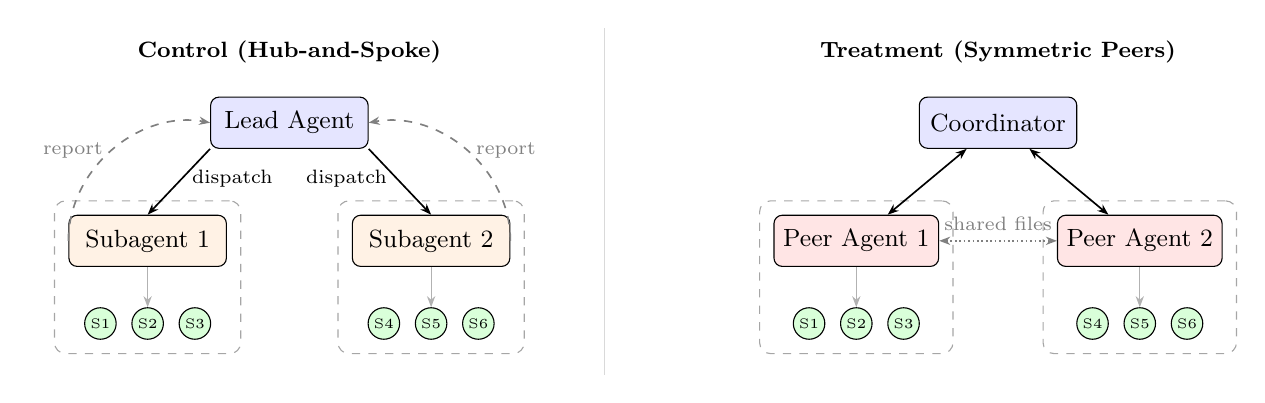
\begin{tikzpicture}[
    agent/.style={draw, rounded corners=3pt, minimum width=2cm,
      minimum height=0.65cm, font=\small},
    sbox/.style={draw, rounded corners=4pt, dashed, gray!70,
      inner sep=5pt},
    sh/.style={draw, circle, minimum size=0.4cm, font=\tiny,
      inner sep=0.5pt, fill=green!15},
    arr/.style={-{Stealth[length=4pt]}, semithick},
    darr/.style={{Stealth[length=4pt]}-{Stealth[length=4pt]}, semithick},
    lbl/.style={font=\footnotesize\bfseries},
  ]
    % ═══ Control (left half) ═══
    \node[lbl] at (-4.5, 3.4) {Control (Hub-and-Spoke)};
    \node[agent, fill=blue!10] (lead) at (-4.5, 2.5) {Lead Agent};

    % Subagent 1 + stakeholders
    \node[agent, fill=orange!10] (sub1) at (-6.3, 1.0) {Subagent 1};
    \node[sh] (s1) at (-6.9, -0.05) {S1};
    \node[sh] (s2) at (-6.3, -0.05) {S2};
    \node[sh] (s3) at (-5.7, -0.05) {S3};
    \node[sbox, fit=(sub1)(s1)(s2)(s3)] (box1) {};

    % Subagent 2 + stakeholders
    \node[agent, fill=orange!10] (sub2) at (-2.7, 1.0) {Subagent 2};
    \node[sh] (s4) at (-3.3, -0.05) {S4};
    \node[sh] (s5) at (-2.7, -0.05) {S5};
    \node[sh] (s6) at (-2.1, -0.05) {S6};
    \node[sbox, fit=(sub2)(s4)(s5)(s6)] (box2) {};

    % Control arrows — dispatch on inner side, report on outer side
    \draw[arr] (lead.south west) --
      node[right, font=\scriptsize, pos=0.45] {dispatch} (sub1.north);
    \draw[arr] (lead.south east) --
      node[left, font=\scriptsize, pos=0.45] {dispatch} (sub2.north);
    \draw[arr, dashed, gray] (sub1.west) to[bend left=50]
      node[left, font=\scriptsize, text=gray, pos=0.5] {\;report} (lead.west);
    \draw[arr, dashed, gray] (sub2.east) to[bend right=50]
      node[right, font=\scriptsize, text=gray, pos=0.5] {report\;} (lead.east);
    \draw[arr, thin, gray!60] (sub1) -- (s2);
    \draw[arr, thin, gray!60] (sub2) -- (s5);

    % ═══ Treatment (right half) ═══
    \node[lbl] at (4.5, 3.4) {Treatment (Symmetric Peers)};
    \node[agent, fill=blue!10] (coord) at (4.5, 2.5) {Coordinator};

    % Peer 1 + stakeholders
    \node[agent, fill=red!10] (peer1) at (2.7, 1.0) {Peer Agent 1};
    \node[sh] (t1) at (2.1, -0.05) {S1};
    \node[sh] (t2) at (2.7, -0.05) {S2};
    \node[sh] (t3) at (3.3, -0.05) {S3};
    \node[sbox, fit=(peer1)(t1)(t2)(t3)] (tbox1) {};

    % Peer 2 + stakeholders
    \node[agent, fill=red!10] (peer2) at (6.3, 1.0) {Peer Agent 2};
    \node[sh] (t4) at (5.7, -0.05) {S4};
    \node[sh] (t5) at (6.3, -0.05) {S5};
    \node[sh] (t6) at (6.9, -0.05) {S6};
    \node[sbox, fit=(peer2)(t4)(t5)(t6)] (tbox2) {};

    % Treatment arrows
    \draw[darr] (coord) -- (peer1);
    \draw[darr] (coord) -- (peer2);
    \draw[darr, densely dotted, gray] (peer1) --
      node[above, font=\scriptsize, text=gray] {shared files} (peer2);
    \draw[arr, thin, gray!60] (peer1) -- (t2);
    \draw[arr, thin, gray!60] (peer2) -- (t5);

    % Divider
    \draw[gray!30, thin] (-0.5, -0.7) -- (-0.5, 3.7);
  \end{tikzpicture}
  \caption{Architecture conditions. \textbf{Left:} Hub-and-spoke---lead
    dispatches subagents that interview stakeholders, return reports,
    and terminate. \textbf{Right:} Symmetric peers are long-lived,
    share a filesystem, and receive coordinator-mediated relay.
    Dashed boxes group each agent with its assigned stakeholders.
    Both conditions use two agents plus a coordinator/lead.}
  \label{fig:architecture}
\end{figure}

\subsection{Partition Conditions}

The six stakeholders form a conflict graph with natural clusters. By
reassigning stakeholders across the agent boundary, we vary how many
of the 8 conflicts require cross-agent information.

\textbf{Partition~A} (low cross-dependency): Agent~1 receives
\{Security Officer, Compliance Lead, EU~Ops\}; Agent~2 receives
\{APAC~Ops, Platform Architect, Product Manager\}. This yields 6
within-partition and 2 cross-partition conflicts (75/25 split). Most
conflicts are resolvable by one agent alone.

\textbf{Partition~C} (high cross-dependency): Agent~1 receives
\{Security Officer, Compliance Lead, Platform Architect\}; Agent~2
receives \{EU~Ops, APAC~Ops, Product Manager\}. This yields 2
within-partition and 6 cross-partition conflicts (25/75 split).
Most conflicts require both agents' information.

Partition~B (50/50) was designed but omitted after piloting:
with $n = 8$ per cell, a predictable midpoint adds less statistical
value than deepening each extreme.

\begin{figure}[t]
  \centering
  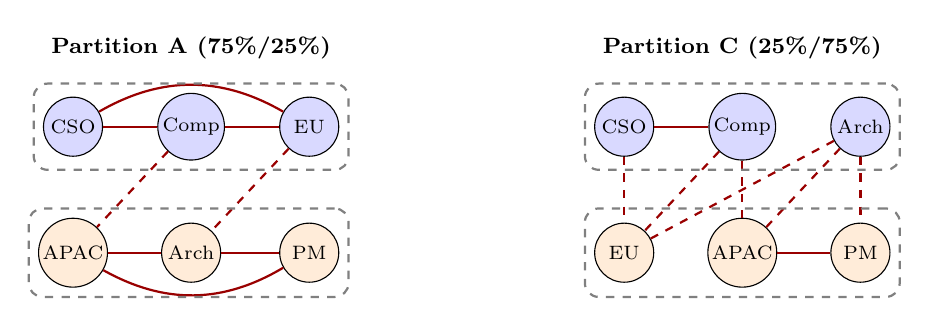
\begin{tikzpicture}[
    snode/.style={draw, circle, minimum size=0.75cm, font=\scriptsize, inner sep=1pt},
    conflict/.style={thick, red!60!black},
    cross/.style={thick, red!60!black, dashed},
    partition/.style={draw, dashed, rounded corners=5pt, gray, thick},
    label/.style={font=\footnotesize\bfseries},
  ]
    % ── Partition A (left) ──
    \node[label] at (-3.5, 2.8) {Partition A (75\%/25\%)};
    \node[snode, fill=blue!15] (a-cso) at (-5, 1.8) {CSO};
    \node[snode, fill=blue!15] (a-comp) at (-3.5, 1.8) {Comp};
    \node[snode, fill=blue!15] (a-eu) at (-2, 1.8) {EU};
    \node[snode, fill=orange!15] (a-apac) at (-5, 0.2) {APAC};
    \node[snode, fill=orange!15] (a-arch) at (-3.5, 0.2) {Arch};
    \node[snode, fill=orange!15] (a-pm) at (-2, 0.2) {PM};
    % Within-partition conflicts (solid)
    \draw[conflict] (a-cso) -- (a-comp);
    \draw[conflict] (a-cso) to[bend left=30] (a-eu);
    \draw[conflict] (a-comp) -- (a-eu);
    \draw[conflict] (a-apac) -- (a-arch);
    \draw[conflict] (a-apac) to[bend right=30] (a-pm);
    \draw[conflict] (a-arch) -- (a-pm);
    % Cross-partition conflicts (dashed)
    \draw[cross] (a-comp) -- (a-apac);
    \draw[cross] (a-eu) -- (a-arch);
    % Partition boxes
    \node[partition, fit=(a-cso)(a-comp)(a-eu), label={[font=\scriptsize]below left:Agent 1}] {};
    \node[partition, fit=(a-apac)(a-arch)(a-pm), label={[font=\scriptsize]above left:Agent 2}] {};

    % ── Partition C (right) ──
    \node[label] at (3.5, 2.8) {Partition C (25\%/75\%)};
    \node[snode, fill=blue!15] (c-cso) at (2, 1.8) {CSO};
    \node[snode, fill=blue!15] (c-comp) at (3.5, 1.8) {Comp};
    \node[snode, fill=blue!15] (c-arch) at (5, 1.8) {Arch};
    \node[snode, fill=orange!15] (c-eu) at (2, 0.2) {EU};
    \node[snode, fill=orange!15] (c-apac) at (3.5, 0.2) {APAC};
    \node[snode, fill=orange!15] (c-pm) at (5, 0.2) {PM};
    % Within-partition conflicts (solid)
    \draw[conflict] (c-cso) -- (c-comp);
    \draw[conflict] (c-apac) -- (c-pm);
    % Cross-partition conflicts (dashed)
    \draw[cross] (c-cso) -- (c-eu);
    \draw[cross] (c-comp) -- (c-eu);
    \draw[cross] (c-comp) -- (c-apac);
    \draw[cross] (c-eu) -- (c-arch);
    \draw[cross] (c-apac) -- (c-arch);
    \draw[cross] (c-arch) -- (c-pm);
    % Partition boxes
    \node[partition, fit=(c-cso)(c-comp)(c-arch), label={[font=\scriptsize]below left:Agent 1}] {};
    \node[partition, fit=(c-eu)(c-apac)(c-pm), label={[font=\scriptsize]above left:Agent 2}] {};
  \end{tikzpicture}
  \caption{Partition conditions showing conflict graph.
    Solid lines: within-partition conflicts (resolvable by one agent).
    Dashed lines: cross-partition conflicts (require both agents' information).
    \textbf{Left:} Partition~A has 6 within / 2 cross.
    \textbf{Right:} Partition~C has 2 within / 6 cross.}
  \label{fig:partitions}
\end{figure}

\subsection{Execution}

\begin{table}[t]
  \caption{Experimental matrix.}
  \label{tab:matrix}
  \centering\small
  \begin{tabular}{lcccr}
    \toprule
    \textbf{Cell} & \textbf{Architecture} & \textbf{Partition}
      & \textbf{Within/Cross} & \textbf{n} \\
    \midrule
    Control-A   & Hub-and-spoke   & A & 6/2 (75\%/25\%) & 8 \\
    Control-C   & Hub-and-spoke   & C & 2/6 (25\%/75\%) & 8 \\
    Treatment-A & Symmetric peers & A & 6/2 (75\%/25\%) & 8 \\
    Treatment-C & Symmetric peers & C & 2/6 (25\%/75\%) & 8 \\
    \midrule
    \textbf{Total} & & & & \textbf{32} \\
    \bottomrule
  \end{tabular}
\end{table}

All 32 runs were conducted as interactive Claude Code sessions using
Claude Opus 4.6 as the agent model. A 30-minute soft time cap was applied.
Each run was self-contained with no cumulative state. Runs were executed
under a Claude Max subscription (\$0 marginal API cost for agent
sessions); stakeholder simulation costs totaled approximately \$1--2.


%═══════════════════════════════════════════════════════════════════
\section{Evaluation Methodology}
\label{sec:eval}
%═══════════════════════════════════════════════════════════════════

We employ two independent evaluation methods to mitigate single-method
bias: a rubric-based assessment with ground-truth items and a blind
architectural review with no rubric knowledge. \Cref{fig:pipeline}
shows the model pipeline: each stage uses a different Claude model to
reduce self-evaluation bias.

\begin{figure}[t]
  \centering
  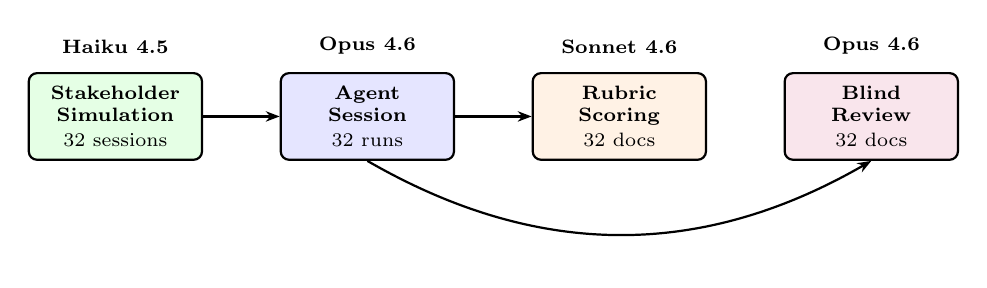
\begin{tikzpicture}[
    stage/.style={draw, rounded corners=3pt, minimum width=2.2cm,
      minimum height=1.1cm, font=\scriptsize, align=center, thick},
    arr/.style={-{Stealth[length=5pt]}, thick},
  ]
    \node[stage, fill=green!10] (sim) at (0, 0)
      {\textbf{Stakeholder}\\\textbf{Simulation}\\[1pt]32 sessions};
    \node[stage, fill=blue!10] (agent) at (3.2, 0)
      {\textbf{Agent}\\\textbf{Session}\\[1pt]32 runs};
    \node[stage, fill=orange!10] (rubric) at (6.4, 0)
      {\textbf{Rubric}\\\textbf{Scoring}\\[1pt]32 docs};
    \node[stage, fill=purple!10] (blind) at (9.6, 0)
      {\textbf{Blind}\\\textbf{Review}\\[1pt]32 docs};

    \node[font=\scriptsize\bfseries, above=3pt] at (sim.north) {Haiku 4.5};
    \node[font=\scriptsize\bfseries, above=3pt] at (agent.north) {Opus 4.6};
    \node[font=\scriptsize\bfseries, above=3pt] at (rubric.north) {Sonnet 4.6};
    \node[font=\scriptsize\bfseries, above=3pt] at (blind.north) {Opus 4.6};

    \draw[arr] (sim) -- (agent);
    \draw[arr] (agent) -- (rubric);
    \draw[arr] (agent.south) to[bend right=30] (blind.south);
  \end{tikzpicture}
  \caption{Evaluation pipeline. Each stage uses a different Claude
    model. Stakeholders are simulated by Haiku~4.5 (temperature~0.2),
    agents are Opus~4.6, rubric scoring uses Sonnet~4.6, and the
    blind review uses a separate Opus~4.6 instance with no rubric
    knowledge.}
  \label{fig:pipeline}
\end{figure}

\subsection{Rubric-Based Evaluation}

A four-layer rubric scores each architecture document against a ground
truth that defines the optimal resolution for each conflict and
dependency:

\begin{itemize}
  \item \textbf{L1 -- Constraint Discovery} (weight 0.25): Did the
    document mention each stakeholder's hard constraints? Scored as a
    checklist (found/not found) via semantic matching.
  \item \textbf{L2 -- Conflict Identification} (weight 0.25): Did the
    document identify the known conflicts between stakeholders? Checklist
    scoring via semantic matching.
  \item \textbf{L3 -- Resolution Quality} (weight 0.30): For each
    identified conflict, how well was it resolved? Scored categorically:
    \emph{Optimal} (1.0)---satisfies both stakeholders' hard constraints
    with minimal preference compromise; \emph{Acceptable} (0.67)---satisfies
    hard constraints but with significant preference trade-offs;
    \emph{Poor} (0.33)---violates one or more hard constraints;
    \emph{Missing} (0.0)---conflict not addressed. Scored by Claude
    Sonnet 4.6 as LLM-as-judge.
  \item \textbf{L4 -- Hidden Dependencies} (weight 0.20): Did the
    document discover non-obvious cross-stakeholder dependencies? Checklist
    scoring via semantic matching.
\end{itemize}

The composite score is the weighted sum:
$\text{Composite} = 0.25 \cdot L1 + 0.25 \cdot L2 + 0.30 \cdot L3 + 0.20 \cdot L4$.

\subsection{Blind Architectural Review}

All 32 architecture documents were independently reviewed by Claude
Opus 4.6 with zero knowledge of the rubric, ground truth, or
experimental conditions. The reviewer scored each document on six
dimensions using a 1--5 scale (total /30):

\begin{enumerate}
  \item \textbf{Internal Consistency (IC):} Do component decisions
    compose without contradictions?
  \item \textbf{Specificity (SP):} Concrete technology choices vs.\
    hand-wavy prose?
  \item \textbf{Buildability (BU):} Could an engineering team implement
    this as written?
  \item \textbf{Trade-off Depth (TD):} Quality of conflict reasoning?
  \item \textbf{Completeness (CO):} Operational concerns, edge cases,
    fallback strategies?
  \item \textbf{Architectural Soundness (AS):} Do patterns fit the
    problem domain?
\end{enumerate}

Documents were reviewed in four batches of eight, with one document per
cell per batch for calibration consistency.

\subsection{LLM-as-Judge: Validity Considerations}
\label{sec:validity}

A core concern is that Claude models evaluate artifacts produced by
Claude agents. The scoring pipeline involves Claude Opus 4.6 agents
producing documents, Claude Sonnet 4.6 scoring the rubric, and Claude
Opus 4.6 conducting the blind review. Three design features mitigate
this concern.

First, \emph{dual-evaluation divergence}: if a systematic bias favoring
treatment outputs existed (e.g., stylistic familiarity), both evaluation
methods would converge on the same individual champions. They do not.
In three of four cells, the rubric champion and the blind review champion
are different runs (\cref{sec:cross-validation}). The methods agree on
the \emph{direction} of the treatment effect but disagree on which
individual documents are best, suggesting they measure genuinely
different qualities.

Second, Layers L1, L2, and L4 of the rubric are essentially
\emph{checklist-based}: does the document mention item~$X$?
This reduces the subjective latitude available to the scorer.
Only L3 (resolution quality) requires open-ended judgment.

Third, the blind review was \emph{uninstructed}: the reviewer received
no rubric, no ground truth, and no scoring criteria. The six dimensions
emerged from the reviewer's own assessment framework, providing an
independent signal.

We acknowledge that these mitigations do not eliminate the possibility
of systematic bias. An independent human evaluation would further
strengthen the findings.


%═══════════════════════════════════════════════════════════════════
\section{Results}
\label{sec:results}
%═══════════════════════════════════════════════════════════════════

\subsection{Architecture Main Effect}
\label{sec:main-effect}

\Cref{tab:main-effect} reports the architecture main effect (Treatment
vs.\ Control, pooled across partitions). Mann-Whitney $U$ tests are used
throughout due to the ordinal nature of rubric scores and small sample
sizes~\cite{mann1947test}. Effect sizes are Cohen's $d$~\cite{cohen1988statistical}.

\begin{table}[t]
  \caption{Architecture main effect (Treatment vs.\ Control, $n = 16$ each).}
  \label{tab:main-effect}
  \centering\small
  \begin{tabular}{lccccc}
    \toprule
    \textbf{Metric} & \textbf{Control} & \textbf{Treatment}
      & $U$ & $p$ & $d$ \\
    \midrule
    Composite       & $0.63 \pm 0.17$ & $0.80 \pm 0.18$ & 62.0  & 0.014\sig & $+0.99$ \\
    L2 Conflict ID  & $0.53 \pm 0.30$ & $0.79 \pm 0.28$ & 63.0  & 0.013\sig & $+0.88$ \\
    L3 Resolution   & $0.41 \pm 0.18$ & $0.64 \pm 0.26$ & 60.0  & 0.011\sig & $+1.04$ \\
    L4 Hidden Deps  & $0.64 \pm 0.33$ & $0.83 \pm 0.27$ & 83.5  & 0.077\msig & $+0.62$ \\
    \bottomrule
  \end{tabular}
  \par\smallskip
  {\footnotesize \sig$p < 0.05$\quad \msig$p < 0.10$}
\end{table}

L1 (Constraint Discovery) shows a ceiling in all four cells
($\geq 0.98$), confirming that both topologies effectively elicit
basic stakeholder requirements. This L1 ceiling serves as a
manipulation check: both topologies successfully extract stakeholder
information, confirming that differences in L2--L4 arise from how
agents \emph{synthesize} across stakeholders, not from differential
information access. The treatment advantage concentrates in L2--L4:
the layers that require cross-stakeholder information synthesis. The largest effect is in L3 (Resolution Quality, \deff{+1.04},
\pval{0.011})---the most demanding layer, requiring agents to
synthesize conflicting requirements into a coherent architectural
resolution. The widest pairwise contrast, Control-A vs.\
Treatment-C, yields \deff{+1.67} (composite) and \deff{+2.13}
(L3)---the full range of the experimental design from lowest
information asymmetry with hub-and-spoke to highest information
asymmetry with peer agents.

\begin{figure}[t]
  \centering
  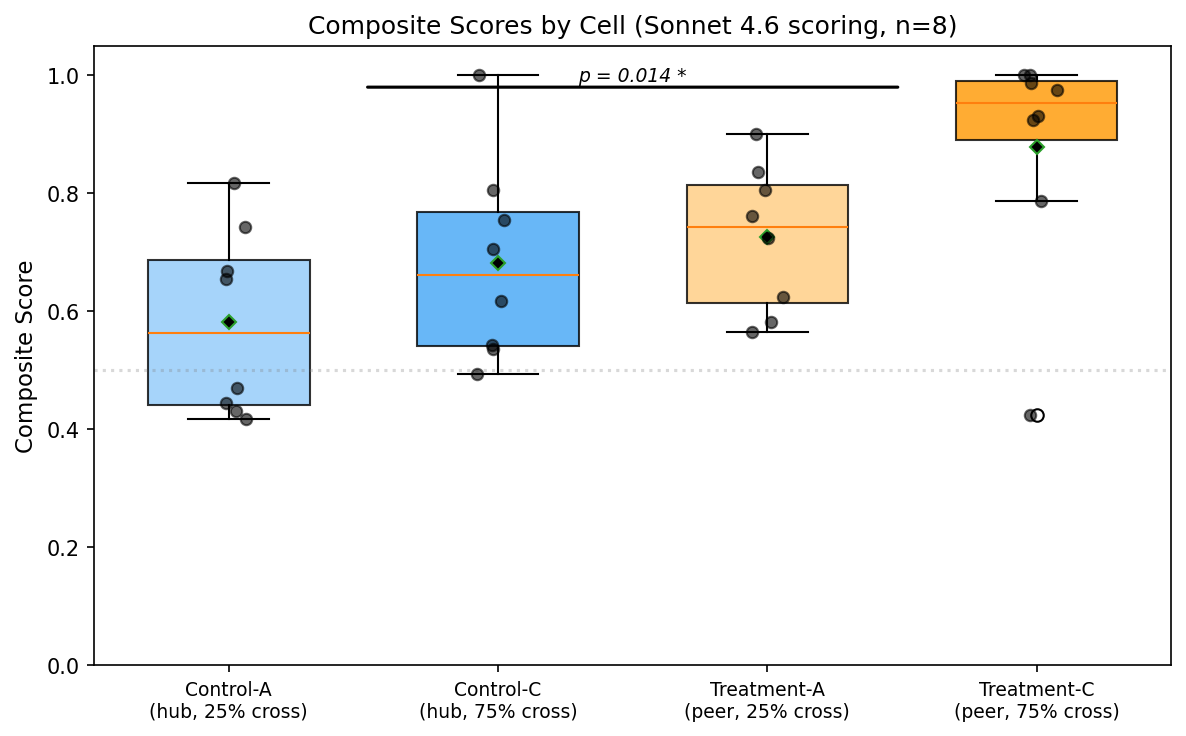
\includegraphics[width=0.85\linewidth]{figures/composite_boxplot.png}
  \caption{Composite score distributions by experimental cell.
    Treatment conditions (right) consistently outperform their control
    counterparts, with the largest separation in Partition~C.}
  \label{fig:composite-boxplot}
\end{figure}

\subsection{Dose-Response}
\label{sec:dose-response}

\Cref{tab:dose-response} decomposes the treatment effect by partition
condition. If information asymmetry is the mechanism, the treatment
advantage should be larger in Partition~C (75\% cross-partition
conflicts) than in Partition~A (25\%).

\begin{table}[t]
  \caption{Dose-response: treatment effect by partition condition.}
  \label{tab:dose-response}
  \centering\small
  \begin{tabular}{lcccc}
    \toprule
    \textbf{Metric} & \textbf{Effect in A} & \textbf{Effect in C}
      & \textbf{Gradient} & \textbf{Interaction $p$} \\
    \midrule
    Composite  & $+0.14$ & $+0.20$ & $+0.05$ & 0.690 \\
    L2         & $+0.28$ & $+0.23$ & $-0.05$ & 0.887 \\
    L3         & $+0.10$ & $+0.36$ & $+0.25$ & 0.129\msig \\
    \bottomrule
  \end{tabular}
  \par\smallskip
  {\footnotesize Interaction $p$ from 100{,}000-permutation test.
  \msig$p < 0.15$, directionally consistent with H2.}
\end{table}

The L3 dose-response pattern is striking: the treatment advantage for
resolution quality is 3.5$\times$ larger in Partition~C ($+0.36$) than
in Partition~A ($+0.10$). The interaction term (\pval{0.129}) does
not reach conventional significance at $n = 8$ per cell, but the
gradient is monotonic and directionally consistent with H2. Power
analysis suggests $n \approx 12$--16 per cell would be needed to
detect this interaction at $\alpha = 0.05$.

L2 (Conflict Identification) shows a \emph{flat} gradient: the treatment
advantage for identifying conflicts is similar regardless of partition.
This is consistent with the mechanism---both topologies can identify
conflicts, but \emph{resolving} cross-partition conflicts specifically
benefits from the peer topology's information flow.

\begin{figure}[t]
  \centering
  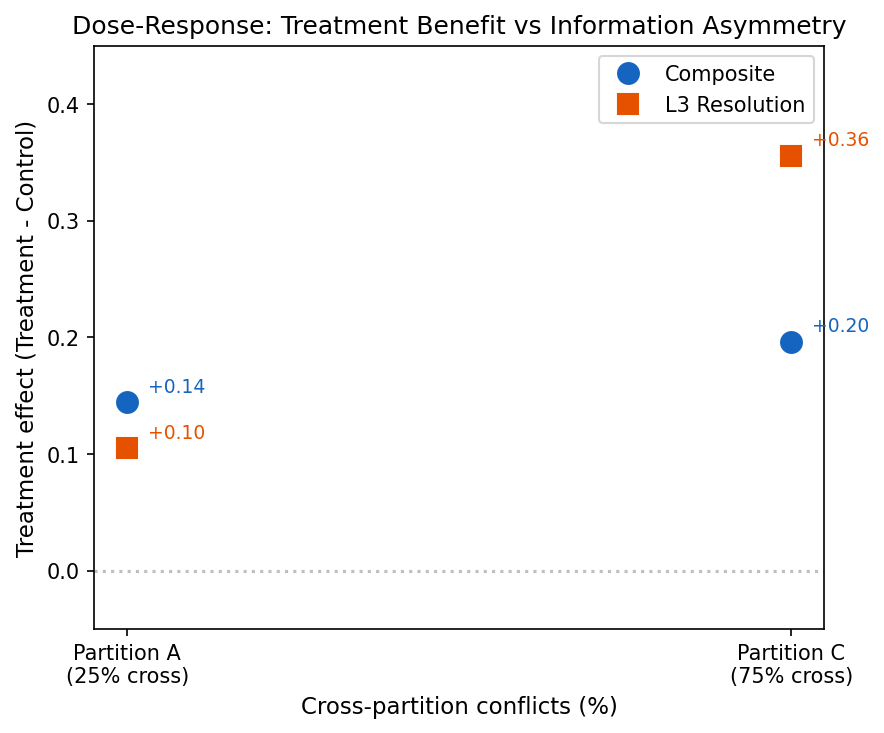
\includegraphics[width=0.85\linewidth]{figures/dose_response.png}
  \caption{Dose-response gradient. The treatment advantage in L3
    (Resolution Quality) is $3.5\times$ larger in Partition~C
    (high cross-partition conflict density) than in Partition~A,
    consistent with an information-asymmetry mechanism.}
  \label{fig:dose-response}
\end{figure}

\subsection{Resolution Quality Breakdown}

Treatment-C achieves L3~$\geq 0.88$ in 5 of 8 runs, a level of
resolution quality never observed in any other cell (except a single
outlier, Control-C-7, at 1.00). Treatment-C runs 1--3 average 7.0
\emph{Optimal} resolutions out of 8 conflicts, compared to 1--2
\emph{Optimal} in Control cells.

Treatment-C also exhibits the highest variance (SD~0.27 on L3).
When peer coordination works well, it works exceptionally (L3~$\geq 0.88$
in 5/8 runs). When it fails, output degrades below the control floor
(runs 4--5: L3 = 0.67 and 0.21). The hub-and-spoke topology trades
ceiling for consistency.

\begin{figure}[t]
  \centering
  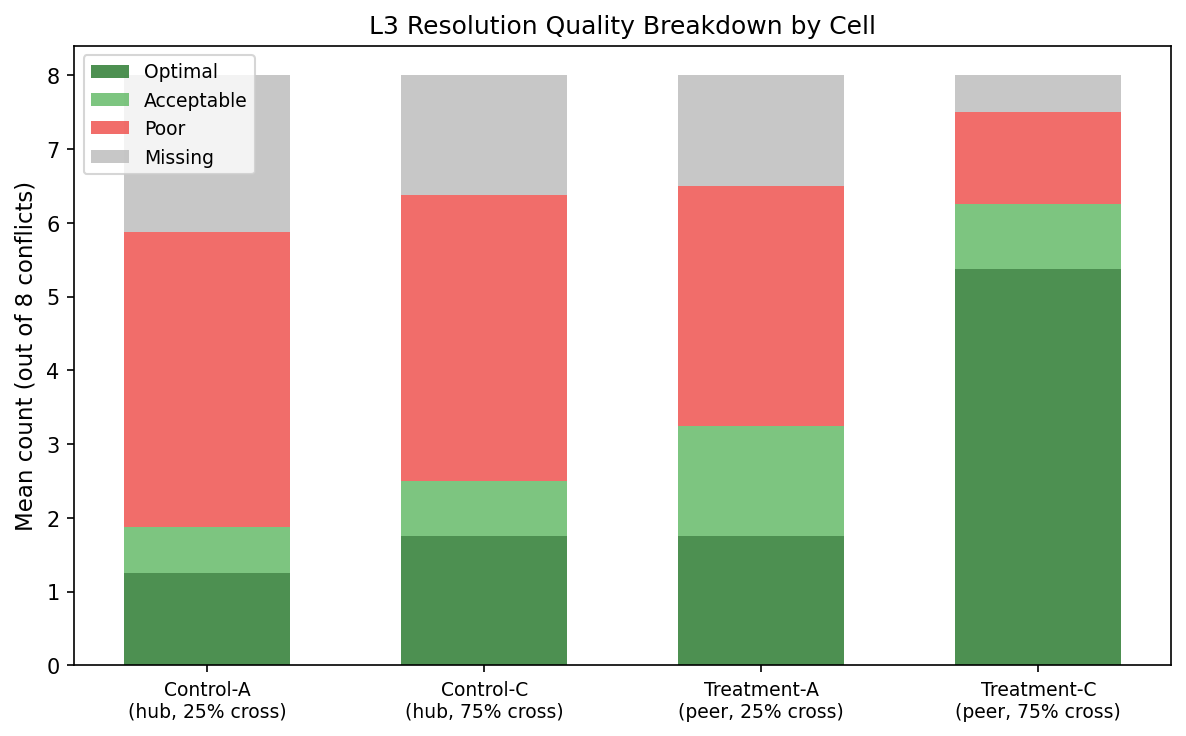
\includegraphics[width=0.85\linewidth]{figures/l3_breakdown.png}
  \caption{L3 (Resolution Quality) per-run breakdown. Treatment-C
    achieves $\geq 0.88$ in 5/8 runs---a level never reached by other
    cells except a single outlier (Control-C-7). Treatment-C also shows
    the highest variance, reflecting the bimodal outcome distribution
    of peer coordination.}
  \label{fig:l3-breakdown}
\end{figure}

\subsection{Blind Architectural Review}

The blind review confirms the rubric's direction. Treatment documents
score $23.9 \pm 2.2$ out of 30, compared to $22.3 \pm 1.2$ for
control ($\Delta = +1.7$).

\begin{table}[t]
  \caption{Blind review per-dimension means (1--5 scale).}
  \label{tab:blind}
  \centering\small
  \begin{tabular}{lccc}
    \toprule
    \textbf{Dimension} & \textbf{Control} & \textbf{Treatment}
      & $\Delta$ \\
    \midrule
    Internal Consistency  & 4.00 & 3.94 & $-0.06$ \\
    Specificity           & 3.31 & 4.06 & $+0.75$ \\
    Buildability          & 3.13 & 3.56 & $+0.44$ \\
    Trade-off Depth       & 4.00 & 4.31 & $+0.31$ \\
    Completeness          & 3.88 & 4.19 & $+0.31$ \\
    Architectural Soundness & 3.94 & 3.88 & $-0.06$ \\
    \bottomrule
  \end{tabular}
\end{table}

The treatment advantage concentrates in three dimensions:
\emph{Specificity} ($+0.75$)---treatment documents name concrete
technologies, provide latency budgets, and specify deployment
topologies where control documents hedge with ``or equivalent'';
\emph{Buildability} ($+0.44$)---treatment documents are sprint-ready
while control documents require another design round; and
\emph{Completeness} ($+0.31$)---treatment documents surface more hidden
dependencies and edge cases. Internal Consistency and Architectural
Soundness show ceiling effects at $\sim$4/5, providing no discrimination.

\subsection{Cross-Validation of Evaluation Methods}
\label{sec:cross-validation}

The rubric and blind review measure different qualities and pick
different individual champions in three of four cells.
For example, Control-C-7 achieves a perfect rubric composite of 1.00
(every conflict identified and optimally resolved) but scores only
22/30 on the blind review---a checklist-compliant document that lacks
engineering specificity. Conversely, Treatment-C-4 scores 0.79 on the
rubric but achieves 27/30 on the blind review (tied highest in the
experiment)---a detailed, buildable document that the rubric
undervalues because its strength lies in dimensions the rubric does
not capture.

Both methods agree that Treatment-C is the best cell and Control-A is
the worst. This convergence on direction, combined with divergence on
individual rankings, strengthens confidence that the treatment effect
is not an artifact of either evaluation method.

\begin{figure}[t]
  \centering
  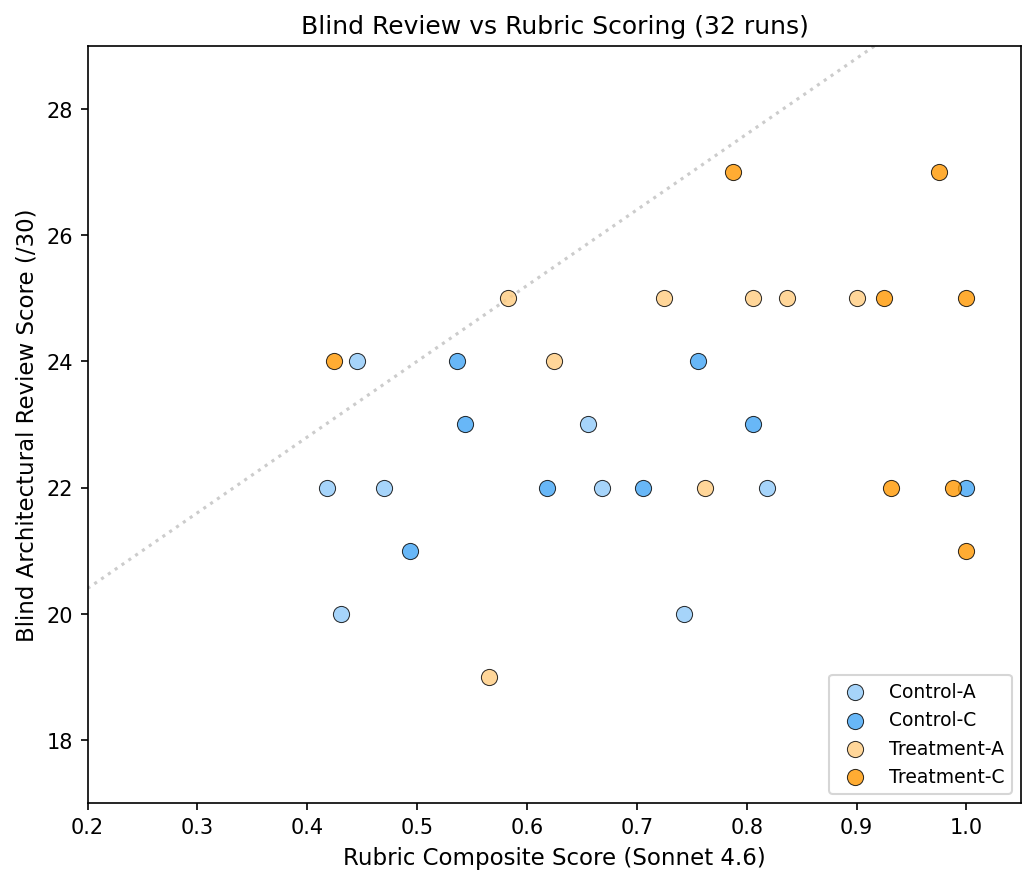
\includegraphics[width=0.85\linewidth]{figures/blind_vs_rubric.png}
  \caption{Cross-validation between rubric-based and blind review
    evaluations. Both methods agree on cell-level direction (Treatment-C
    best, Control-A worst) but select different individual champions,
    indicating complementary rather than redundant evaluation.}
  \label{fig:blind-vs-rubric}
\end{figure}


%═══════════════════════════════════════════════════════════════════
\section{Discussion}
\label{sec:discussion}
%═══════════════════════════════════════════════════════════════════

\subsection{The Zero-Direct-Messages Finding}

Across all three experiments---24 bug-fixing runs, 24 feature
implementation runs, and 32 architecture design runs---agents
\emph{never} used the \texttt{SendMessage} tool to communicate directly
with a peer agent. All inter-agent information flow in treatment runs
was coordinator-mediated: an agent reports findings to the coordinator,
the coordinator relays relevant information to the other agent. We
reconstructed these mediated exchanges by temporal adjacency and
directionality in the transcript (Agent~1 $\to$ Coordinator immediately
followed by Coordinator $\to$ Agent~2).

Yet the treatment significantly outperforms the control. This implies
the advantage is \emph{topological}, not \emph{behavioral}:

\begin{enumerate}
  \item \textbf{Long-lived agents:} Peer agents persist throughout the
    session and can be re-queried. Subagents terminate after returning
    a report, preventing iterative refinement.
  \item \textbf{Shared file context:} Both peer agents read and edit
    the same architecture document. Agent~2 can respond to Agent~1's
    contributions in real time, without the coordinator explicitly
    relaying them.
  \item \textbf{Iterative cross-pollination:} The coordinator relays
    findings between peers, and peers conduct follow-up stakeholder
    interviews informed by the other agent's discoveries. This creates
    a feedback loop absent in the control, where subagents' follow-up
    questions are not informed by the other subagent's findings.
\end{enumerate}

Three communication metrics provide mechanistic evidence for why
the peer topology outperforms. \emph{Relay transparency} measures
whether information from one agent's stakeholder interviews appears
in the other agent's outputs, quantified as the cosine similarity
between interview content embeddings and cross-agent statements.
\emph{Indirect collaboration} detects whether both agents read or
modified the same file (from transcript file operations).
\emph{Message volume} counts coordinator-mediated messages per run.

\begin{table}[t]
  \caption{Communication metrics for treatment cells.}
  \label{tab:comms}
  \centering\small
  \begin{tabular}{lcccc}
    \toprule
    \textbf{Cell} & \textbf{Relay events}
      & \textbf{Mean similarity} & \textbf{Indirect collab.}
      & \textbf{Msg range} \\
    \midrule
    Treatment-A & 3/8 runs & 0.092 & 3/8 runs & 2--13 \\
    Treatment-C & 4/8 runs & 0.276 & 3/8 runs & 3--12 \\
    \bottomrule
  \end{tabular}
\end{table}

Treatment-C shows $3\times$ higher relay similarity than Treatment-A
(0.276 vs.\ 0.092), indicating that when cross-partition information
is relayed in the high-cross condition, it is relayed with greater
fidelity. The four Treatment-C runs with detected relay events are
also the four highest-scoring runs in that cell (composite 0.93--1.00,
relay similarity 0.10--0.42), suggestive of a quality--fidelity
relationship though the sample ($n = 4$) precludes formal testing.

Message volume does \emph{not} predict quality: treatment-C-3
(5~messages, composite 1.00) outperforms treatment-A-7 (13~messages,
composite 0.73). The advantage comes from what is relayed, not how
much.

Indirect collaboration detection rates are low (3/8 in both cells),
but this likely underestimates the true rate: Agent Teams transcripts
do not expose agent-level attribution for file operations, so all
edits appear coordinator-level. The shared file context mechanism
described above likely operates in most or all treatment runs.

\begin{table}[t]
  \caption{Process metrics by cell (mean $\pm$ SD).}
  \label{tab:process}
  \centering\small
  \begin{tabular}{lcccc}
    \toprule
    \textbf{Cell} & \textbf{Wall clock (min)}
      & \textbf{Interviews} & \textbf{Peer msgs}
      & \textbf{Unique pairs} \\
    \midrule
    Control-A   & $8.8 \pm 1.2$  & $8.4 \pm 1.5$  & --- & --- \\
    Control-C   & $10.0 \pm 2.0$ & $13.6 \pm 3.8$ & --- & --- \\
    Treatment-A & $14.6 \pm 3.3$ & $16.4 \pm 5.8$ & $6.8 \pm 3.8$ & $2.1 \pm 0.4$ \\
    Treatment-C & $15.6 \pm 1.8$ & $16.6 \pm 4.7$ & $5.8 \pm 2.7$ & $2.3 \pm 0.5$ \\
    \bottomrule
  \end{tabular}
\end{table}

Treatment runs take 60--75\% longer and involve roughly twice the
stakeholder interviews. This additional process is the mechanism, not
a confound: the peer topology enables a deeper exploration process
(discovery $\to$ relay $\to$ informed follow-up $\to$ synthesis) that
the hub-and-spoke architecture structurally cannot support.
Crucially, additional time alone cannot replicate this process under
hub-and-spoke: subagents terminate after returning reports, so the
lead cannot dispatch informed follow-up interviews---it can only
re-dispatch fresh subagents that lack the other agent's context.

The implication for multi-agent system design is that \emph{channel
availability does not guarantee channel use}. Agents never spontaneously
adopt lateral communication. The advantage comes from the topology's
architectural properties, not from emergent collaborative behavior.

\subsection{What Information Asymmetry Buys}

The three experiments form a natural ablation study:
\begin{itemize}
  \item Experiments~1--2: no information asymmetry $\to$ no quality
    advantage (ceiling effect, zero communication).
  \item Experiment~3: information asymmetry by construction $\to$
    significant quality advantage (\deff{+0.99}).
\end{itemize}

The distinction is not task difficulty. Architecture design is not
inherently ``harder'' than feature implementation---it is
\emph{structurally different} because no single agent holds the
full picture. This is the default condition in real organizations:
different teams hold different knowledge, and high-quality synthesis
requires cross-boundary information transfer. Multi-agent systems
should be evaluated on tasks that reflect this structure.

\subsection{Implications for Practitioners}

\begin{enumerate}
  \item \textbf{Use peer topologies when agents hold asymmetric
    information.} If all agents have full access to the same data,
    subagents are sufficient for parallelism.
  \item \textbf{Do not expect agents to use messaging channels.} In
    80 runs across three experiments, agents never spontaneously sent
    peer messages. If structured communication is needed, build it into
    the protocol, not the channel.
  \item \textbf{The time cost is real.} Treatment runs take 60--75\%
    longer. The quality gain must justify the time cost for a given
    use case.
  \item \textbf{Invest in information design.} The biggest lever for
    multi-agent quality is how information is distributed across agents,
    not how communication channels are configured.
\end{enumerate}

\subsection{Limitations}

\textbf{Single scenario.} All 32 runs use the DataFlow Corp scenario.
Results may not generalize to other domains or conflict structures.

\textbf{Single model.} All agents are Claude Opus 4.6. The treatment
effect may differ for other model families or capability levels.

\textbf{LLM-as-judge.} Despite dual-evaluation divergence (\cref{sec:validity}),
we cannot fully rule out systematic bias from Claude evaluating
Claude-generated artifacts. An independent human evaluation would
strengthen the findings.

\textbf{Small $n$.} With $n = 8$ per cell, the interaction test for
dose-response is underpowered (\pval{0.129}). The main effect
(\pval{0.014}) is significant, but pairwise comparisons between
adjacent cells are not.

\textbf{No Partition~B.} The 50/50 partition was omitted; monotonicity
of the dose-response gradient is assumed but not confirmed.

\textbf{Treatment-C variance.} The peer topology's best and worst
individual-run scores both come from Treatment-C (composite 1.00
and 0.42). Peer coordination has a failure mode that hub-and-spoke
does not.

\textbf{Time confound.} Treatment runs take 60--75\% longer. We
cannot fully disentangle quality improvement from additional
exploration time, though the peer topology produces higher returns
per additional minute than the control.

\textbf{Simulated stakeholders.} LLM-backed stakeholders may be more
predictable than real humans, potentially advantaging the iterative
follow-up process enabled by the treatment topology.

\textbf{Transcript opacity.} Agent Teams does not expose agent-level
attribution for file operations, making indirect collaboration
analysis unreliable. The true volume of inter-agent coordination
is likely higher than our metrics capture.


%═══════════════════════════════════════════════════════════════════
\section{Conclusion}
\label{sec:conclusion}
%═══════════════════════════════════════════════════════════════════

We conducted three experiments comparing symmetric peer agents against
hub-and-spoke subagents on software engineering tasks. The first two
experiments (bug-fixing and feature implementation) produced ceiling
effects with zero inter-agent communication, establishing that
code-level tasks with full information observability provide no
structural advantage for peer coordination. The third experiment
(architecture design with partitioned stakeholders) produced the
first significant result: a large treatment effect (\deff{+0.99},
\pval{0.014}) that scales with cross-partition conflict density
(3.5$\times$ larger advantage at 75\% cross-partition vs.\ 25\%).

The most surprising finding is that agents never use direct peer
messaging despite it being available. The treatment advantage arises
from the topology's architectural properties: long-lived agents,
shared file context, and coordinator-mediated iterative relay. This
reframes the practical recommendation from ``enable agent communication
channels'' to ``design tasks with appropriate information distribution
and use peer topologies for complex synthesis.''

Future work should validate these findings across multiple scenarios
and domains, increase sample sizes to achieve adequate power for
interaction tests, introduce structured deliberation protocols to
test whether explicit peer communication unlocks additional quality
gains, and conduct human evaluation to rule out LLM-as-judge bias.
Beyond the two-agent case studied here, a natural extension is to
deeper agent hierarchies (sub-leads dispatching workers) and hybrid
topologies (peers within clusters, hub-and-spoke between clusters),
testing whether the information asymmetry mechanism scales or whether
coordination overhead eventually dominates. Varying agent count
(4, 8, 16) would clarify how the treatment effect interacts with the
surface area of partition boundaries.
The information asymmetry hypothesis---that it is the distribution
of information, not the difficulty of the task, that determines
whether multi-agent coordination improves quality---provides a
testable framework for guiding these investigations.

%═══════════════════════════════════════════════════════════════════
\bibliographystyle{plain}
\bibliography{references}

\end{document}
